\chapter{Methodology}
\label{sec:Methodology}

This chapter will present the whole procedure of the implemented anaphora resolution system with all of its stages. The complete system can also be examined online.\footnote{The download is available at https://github.com/HenryvanderVegte/henryvdv.BA}


\section{Preprocessing}
\begin{figure}[h]
	\centering

	\fbox{ 
  		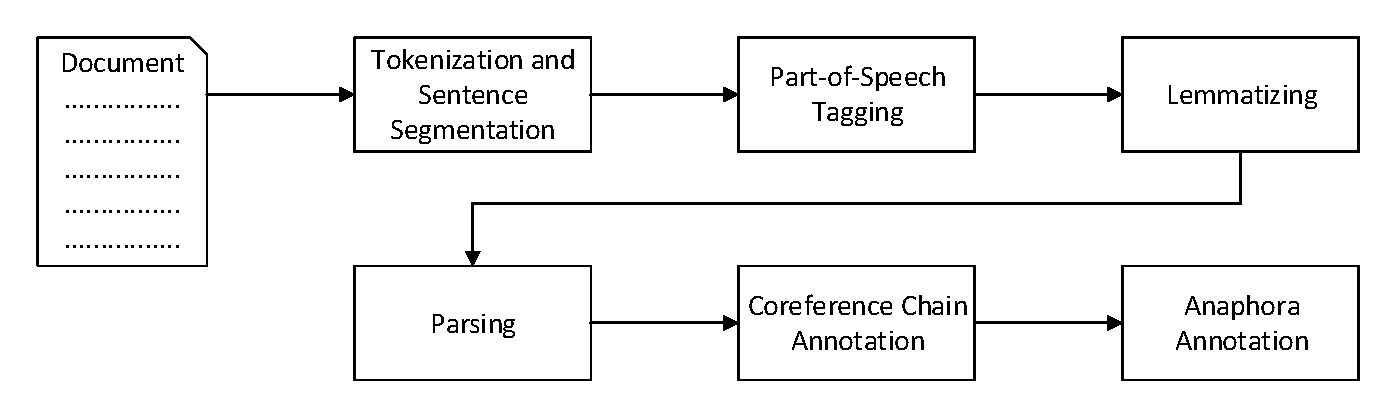
\includegraphics[width=\linewidth]{figures/nlppipelinev2.pdf}
	}	
	\caption{Natural language preprocessing pipeline}
	\label{figure:nlppipeline}
\end{figure}

First of all, the required information of the training corpus need to be extracted. The natural language preprocessing pipeline shown in Table \ref{figure:nlppipeline} was used.  The WikiCoref annotation scheme already includes information on tokens, sentences, and coreferential chains and could easily be extracted.

Still, several other information is missing in order to apply feature values (for instance, information on nominal phrases and part of speech). The \textit{Stanford CoreNLP} toolset \citep{manning-EtAl:2014:P14-5} was used to gain those informations. More precisely, its Part-of-Speech tagger, lemmatizer, named entity recognizer, and parser were applied. 
Note that the assigned labels for the part-of-speech tagger and the parser are simplified in order to reduce complexity of the following examples. For instance, the implemented part-of-speech tagger will differentiate between 
A Part-of-Speech tagger annotates for each token a word class. Word classes are for instance nouns or verbs. Additionally, the tagger differentiates also on more specific details like number or tense. In total, the tagset contains 52 different tags.
The lemmatizer creates for each word its canonical form. A lemma is similar to the word stem, but focuses of the use of the word while most stemmers mostly remove the end of the word to receive its word stem\footnote{http://nlp.stanford.edu/IR-book/html/htmledition/stemming-and-lemmatization-1.html}.
The named entity recognizer identifies amongst others persons, organizations, and dates. \\
An illustrative example of these elements is shown in Figure \ref{figure:nlppipelineexample}. 

\begin{figure}[h]
	\centering
	\fbox{ 
  		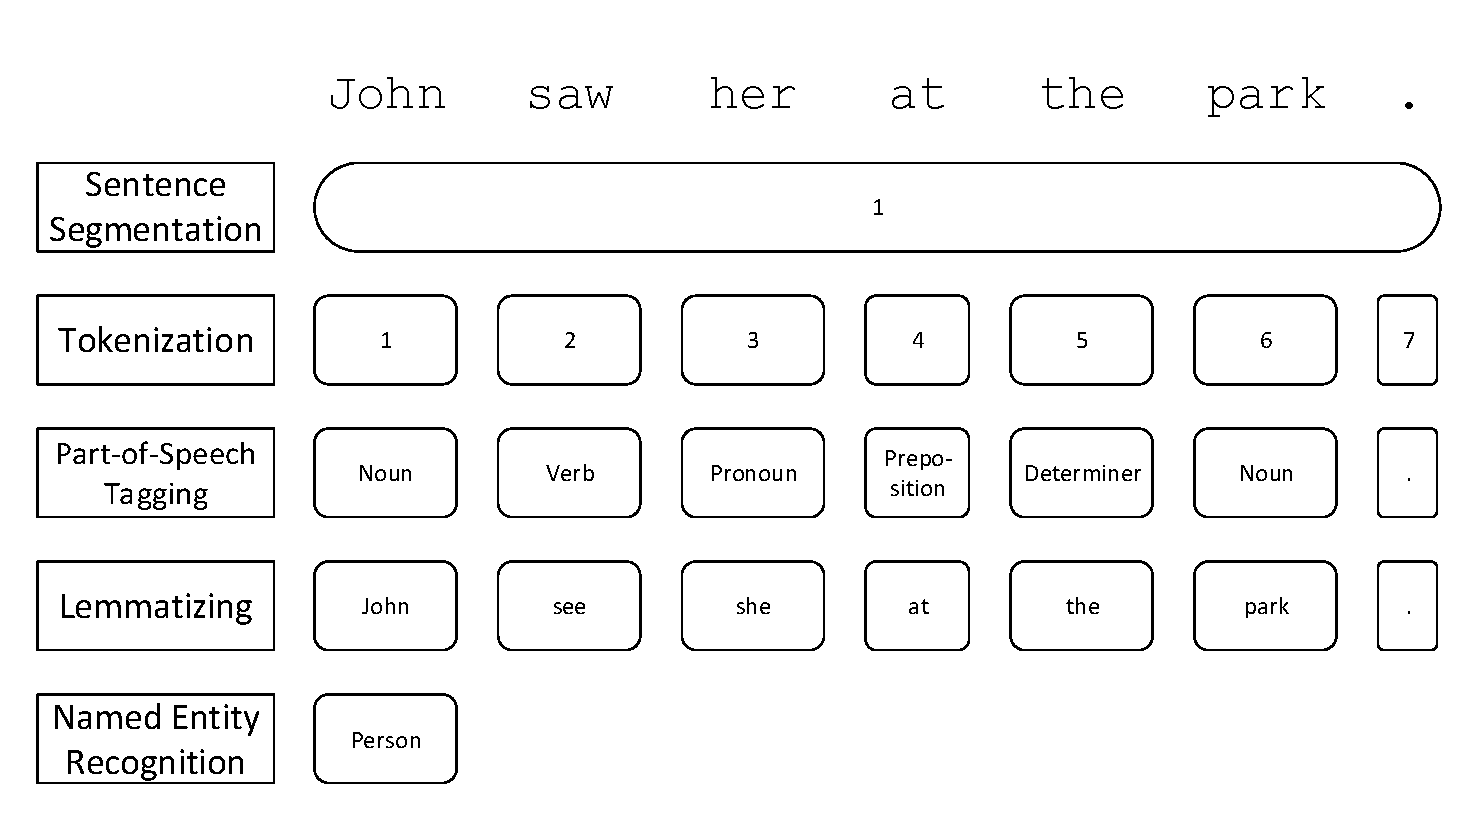
\includegraphics[width=\linewidth]{figures/pipelineExample3.pdf}
	}	
	\caption{Annotation example}
	\label{figure:nlppipelineexample}
\end{figure}

The Parser can be subdivided in two different modules named constituent parser and dependency parser. 

The constituent parser divides the sentence into sub-phrases in an hierarchical order. The type of the phrase is defined by the central word in it (also called head word) \citep{jurafsky2014speech}. For instance, if the head word is a noun the considered phrase is called noun-phrase. The most common kind of illustration is through a dependency parsed tree as shown in Figure \ref{figure:constituencytree}.

The dependency parser describes the relationship of words among each other. A word that is dependent of another is linked directed to it. Additionally, the relationship between both words is annotated. Most graphic representation visualize the relationship through pointed arrows based on the dependent word. An exemplary dependency parsed model is shown in Figure \ref{figure:dependencytree}. The arrow description will thereby represent the type of the relationship. The abbreviations subj., mod., obj., and det. represent subjects, modifiers, object, and determiners.

\begin{figure}[h]
	\centering
	\fbox{ 
  		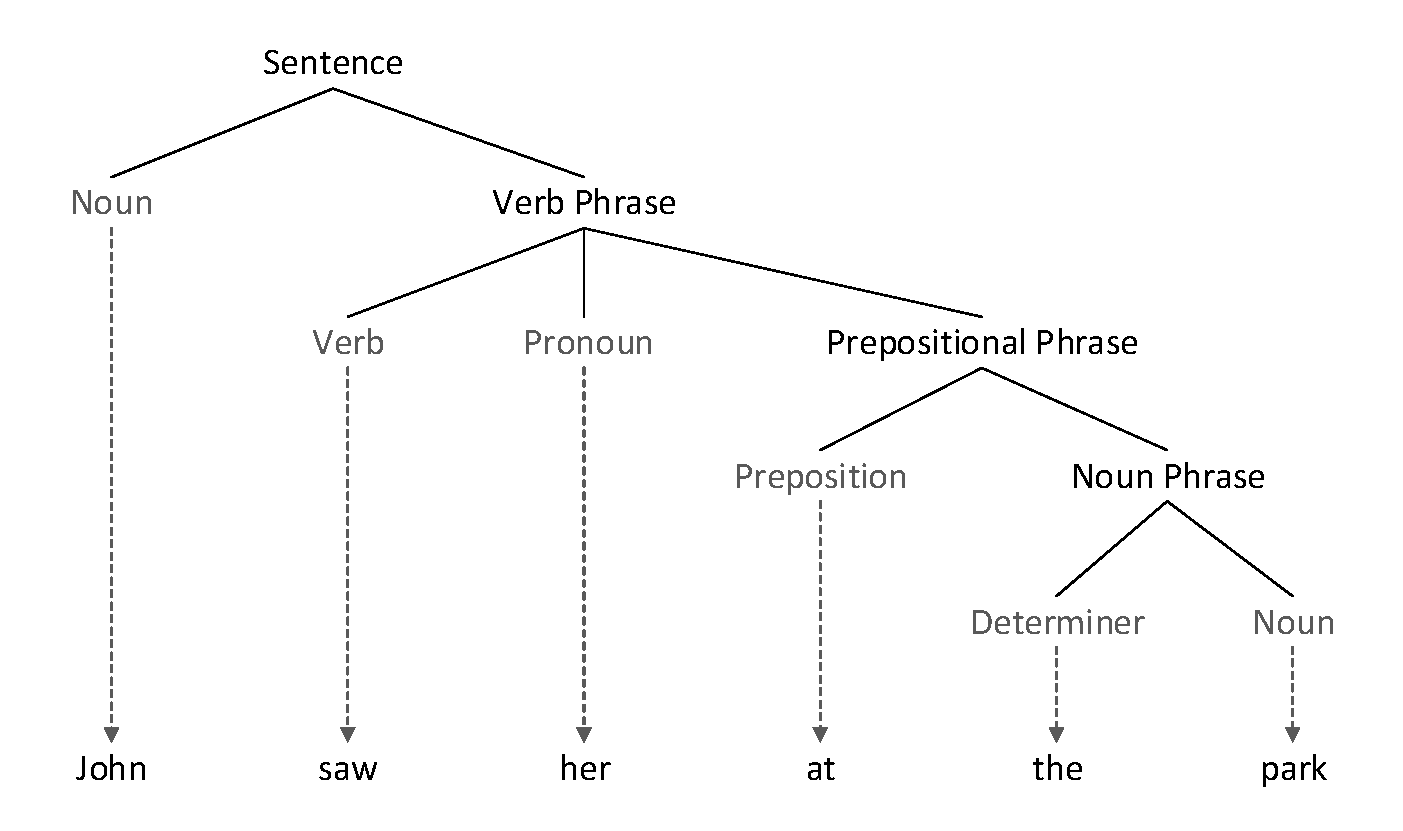
\includegraphics[width=\linewidth]{figures/constituencyTree2.pdf}
	}	
	\caption{Constituency-based parse tree example}
	\label{figure:constituencytree}
\end{figure}

\begin{figure}[h]
	\centering
	\fbox{
	\scalebox{1.7}{ 
\begin{dependency}[theme = simple,thick]
   \begin{deptext}[column sep=1em]
 	 John \& saw  \& her  \& at  \& the  \& park  \\
   \end{deptext}
   \deproot{2}{root}
   \depedge{2}{1}{subj.}
   \depedge[edge start x offset=-2pt]{2}{6}{mod.}
   \depedge{2}{3}{obj.}
   \depedge[arc angle=50]{6}{5}{det.}
   \depedge{6}{4}{case}
\end{dependency}
	}	
}
	\caption{Dependency parsed example}
	\label{figure:dependencytree}
\end{figure}

Coreferential information in WikiCoref is stored through a joint identification number for each coreferring annotation and can therefore be easily extracted. The third person pronominal anaphoras were extracted of the coreference chain as follows: For each pronoun in the current document, search the preceding phrase of its coreference chain. The pronoun will be tagged as the anaphora and the preceding phrase as the antecedent. 

As soon as all relevant information is annotated, a training set needs to be created. In order to do so, the procedure \cite{soon2001machine} was adopted. As already stated in Section \ref{soon2001traininginstances}, all anaphoras and their respective antecedents form thereby positive feature vectors while all intermediate noun phrases form negative feature vectors with their respective anaphoras. For instance, a sequence of noun phrases A-B-C-D with A coreferring D and D as pronoun is considered. In this case the pair (A,D) forms a positive instance while (C,D) and (B,D) form negative instances.\\
The idea of selecting that approach is as follows: All intermediate noun phrases must be clearly not the antecedent so that a human can reject them. In contrast, noun phrases %follows train of thought

%Der Ansatz wurde ausgewählt, da: 1. Alle Sätze müssen für einen Menschen verständlich sein, das heißt ein Mensch ist in der Lage zu entscheiden, dass alle dazwischenliegenden phrasen 
\section{Featureset}
asd

\begin{table}[p]
  \begin{tabular}{| l | l | r |}

    \hline
    Feature Type & Feature & Description \\ \hline
\hline

	\multirow{4}{1.3cm}{Pronoun referred} & Masculine & If pronoun is masculine: 1, else: 0 \\ \cline{2-3}
 	& Feminine &  If pronoun is feminine: 1, else: 0 \\	\cline{2-3}
	& Neutral &  If pronoun is neutral: 1, else: 0 \\	\cline{2-3}
	 & Plural & If pronoun is plural: 1, else: 0 \\ \hline
	\hline
	\multirow{17}{1.3cm}{Antecedent referred} & Antecedent Frequency & number of occurences / 10.0 \\ \cline{2-3}
 	& Subject &  If antecedent contains subject: 1, else: 0 \\ \cline{2-3}
	& Object &   If antecedent contains object: 1, else: 0 \\	\cline{2-3}
	& Predicate &   If antecedent contains predicate: 1, else: 0 \\ \cline{2-3}
	& Pronominal &  If antecedent contains pronoun: 1, else: 0 \\	\cline{2-3}
	& Head-Word Emphasis &  If antecedent parent is no noun: 1, else: 0 \\	\cline{2-3}
	& Conjunction &  If antecedent is not part of cunjunction: 1, else: 0 \\	\cline{2-3}
	 & Prenominal modIfier & If antecedent contains prenominal modIfier: 1, else: 0 \\ \cline{2-3}
	& Organization & If antecedent contains organization: 1, else: 0 \\ \cline{2-3}
	& Person & If antecedent contains person: 1, else: 0 \\ \cline{2-3}
	& Time & If antecedent contains time units: 1, else: 0 \\ \cline{2-3}
	& Date & If antecedent contains date: 1, else: 0 \\ \cline{2-3}
	& Money & If antecedent contains monetary name: 1, else: 0 \\ \cline{2-3}
	& Number & If antecedent contains prenominal modIfier: 1, else: 0 \\ \cline{2-3}
	& Definite & If antecedent has definite article: 1, else: 0 \\ \cline{2-3}	
	& His/Her & If antecedents first word is his or her: 1, else: 0 \\ \cline{2-3}
	& He/His & If antecedents first word is he or his: 1, else: 0 \\  \hline
	\hline
	\multirow{9}{1.3cm}{Pronoun and antecedent referred} & Binding Theory & If binding principles B and C are satisfied: 1, else: 0 \\ \cline{2-3}
 	& Same Sentence &  If both are in the same sentence: 1, else: 0 \\	\cline{2-3}
	& Intra-Sentence Diff. &  Difference in sentences / 50.0 \\	\cline{2-3}
	& In Previous Sentence & If antecedent is in previous sentence: 1, else: 0 \\ \cline{2-3}
	& Inter-Sentence Diff. & Difference in tokens / 50.0\\ \cline{2-3}
	& Prepositional Parallel & If both depend on the same preposition: 1, else: 0 \\ \cline{2-3}
	& Quotation Situation & If both are in or out quotes: 1, else: 0 \\ \cline{2-3}
	& Singular Match & If both are singular: 1, else: 0 \\ \cline{2-3}
	& Plural Match & If both are plural: 1, else: 0 \\ \hline
	\hline
	\multirow{11}{1.3cm}{Gender referred} & Standard Gender Match & If gender is known and matches: 1, else: 0 \\ \cline{2-3}
 	& Standard Gender Mismatch &  If gender is known and mismatches: 1, else: 0 \\	\cline{2-3}
	& Pronoun Mismatch &  If both are pronouns and mismatch: 1, else: 0 \\	\cline{2-3}
	& Masculine Mean & $\mu$ of masculine distribution \\ \cline{2-3}
	& Masculine Variance & Variance of masculine distribution \\ \cline{2-3}
	& Feminine Mean & $\mu$ of feminine distribution \\ \cline{2-3}
	& Feminine Variance & Variance of feminine distribution \\ \cline{2-3}
	& Neutral Mean & $\mu$ of neutral distribution \\ \cline{2-3}
	& Neutral Variance & Variance of neutral distribution \\ \cline{2-3}
	& Plural Mean & $\mu$ of plural distribution \\ \cline{2-3}
	& Plural Variance & Variance of plural distribution \\ \hline

  \end{tabular}
  \caption{Pronoun Resolution Feature Set}
\end{table}

\subsection{Pronoun Features}
asd
\subsection{Antecedent Features}

\subsection{Pronoun-Antecedent Features}

\subsection{Gender Features}

\section{Generating Training Instances}

% vergleich von 3 Sachen: 1. Bergsma approach 2.Fmeasure approach mit nur dem vorherigen element 3. Fmeasure mit allen Elementen in der gleichen chain
\section{Baseline Approach}

\section{SVM Classifier}